\scanpage{103}
\begin{verbatim}
*******************************************************************************
*JESNEWS DU 09/08/1982 C68 CADARACHE                                          *
*******************************************************************************
*      DEPUIS LE 1/7/82 LES ALIAS DES COMMANDES LIBRARIAN                     *
*             LIBGET (LG) ET LIBSAVE (LS) SONT SUPPRIMES,                     *
*             POUR EVITER UNE POSSIBILITE DE CONFLIT AVEC                     *
*             LE MEME ALIAS DES COMMANDES STANDARD IBM.                       *
*      ********                                                               *
* ATTENTION                                                                   *
*   MISE EN SERVICE LE VENDREDI 30/7/82 A 8H00 DE LA DEUXIEME PHASE DE GAF    *
*     SUR 168 CADARACHE.                                                      *
*     ELLE PERMET D'UTILISER DANS LA CDE. KEEP TSO ET DANS LA PROCEDURE KEEP  *
*     BATCH UNE POSSIBILITE D'AFFECTATION DE TYPE DE SAUVEGARDE AU NIVEAU DU  *
*     FICHIER.CETTE POSSIBILITE EST VIVEMENT CONSEILLEE.                      *
*     POUR PLUS AMPLES INFORMATIONS VOIR NOTE TECHNIQUE CISI MVS140,LA NOTE   *
*     MVS 143 ETANT SUPPRIMEE.                                                *
*                                                                             *
* EXEMPLES D'UTILISATION:                                                     *
*                                                                             *
*  BATCH:  DSN=NOM.DU.FICHIER.A.SAUVEGARDER,DELAY=TYPE DE SAUVEGARDE          *
*                                                                             *
*  TSO:                                                                       *
*  K DA('NOM DU FICHIER A SAUVEGARDER') DELAY(TYPE DE SAUVEGARDE)             *
*                                                                             *
*  TYPES DE SAUVEGARDE:                                                       *
*                                                                             *
*      W       SAUVEGARDE HEBDO.                                              *
*      D       SAUVEGARDE JOURNALIERE.                                        *
*      NOS     SAUVEGARDE MENSUELLE.                                          *
*      W       PARAMETRE PAR DEFAUT.                                          *
*                                                                             *
*******************************************************************************
\end{verbatim}
\begin{verbatim}
******************************************************************
*                                                                *
*                  - J E S N E W S   F R 1 -      LE 18/08/82    *
*                                                                *
*----------------------------------------------------------------*
*                                                                *
*  DEPUIS LE LUNDI 12 JUILLET 82, LES CLASSES DE TRAVAUX D ET E  *
*  SERONT ETENDUES POUR UNE TAILLE MEMOIRE SUPERIEURE A 1024 K   *
*  SE REPORTER A LA NOTE TECHNIQUE MVS141.                       *
*                                                                *
*----------------------------------------------------------------*
*  A PARTIR DU LUNDI 9 AOUT 1982 , IL SERA POSSIBLE D'IMPRIMER   *
*  SUR XEROX 9700 (DESTINATION SAC) DES FICHIERS UTILISANT LE    *
*  COUPLE DE JEUX DE CARACTERES : (GS15,GT15)                    *
*                                                                *
*----------------------------------------------------------------*
*                                                                *
*-LE 16/08/82 :                                                  *
*----------------------------------------------------------------*
*  -LE 370/168 SERA ARRETE DU VENDREDI 20 AOUT A 19H JUSQU'AU    *
*   LUNDI 23 AOUT A 8H.( MISE A NIVEAU TECHNIQUE.).              *
*                                                                *
*----------------------------------------------------------------*
*                                                                *
*-LE 18/08/82 :                                                  *
*-------------                                                   *
\end{verbatim}
\figure{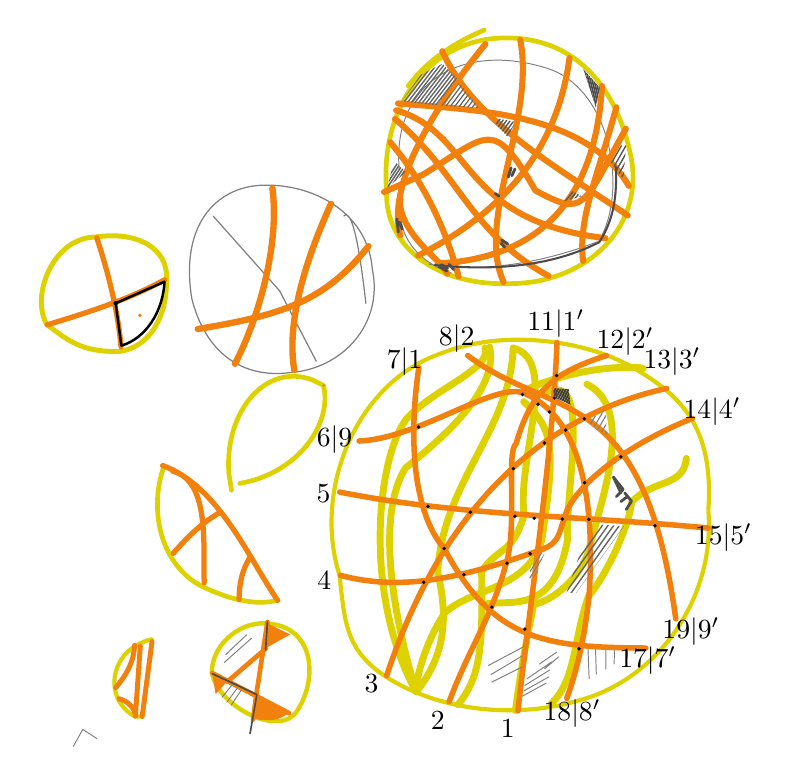
\begin{tikzpicture}[x=.0048cm,y=-.0048cm,line cap=round,line join=round]
\draw[yellow!70!olive,line width=1.7pt] (2020,746)..controls(2000,521)and(2135,339)..(2334,340)..controls(2508,338)and(2622,457)..(2663,642)..controls(2708,832)and(2555,986)..(2351,989)..controls(2135,997)and(2014,877)..(2020,746) (2077,467)..controls(2138,384)and(2226,341)..(2278,319);
\draw[gray,line width=.35pt] (2053,685)..controls(2035,458)and(2219,348)..(2447,421)..controls(2613,477)and(2658,743)..(2582,875) (2063,766)..controls(2038,854)and(2100,932)..(2191,961) (2133,938)..controls(2286,963)and(2451,929)..(2591,873);
\draw[orange!80!brown,line width=2.2pt] (2167,375)..controls(2250,559)and(2457,672)..(2657,809) (2281,356)..controls(2142,527)and(2020,730)..(2056,861) (2373,345)..controls(2414,556)and(2254,819)..(2329,985) (2503,393)..controls(2475,606)and(2358,786)..(2103,915) (2589,467)..controls(2574,723)and(2463,920)..(2155,936) (2627,523)..controls(2573,720)and(2526,817)..(2539,929) (2652,580)..controls(2536,788)and(2545,814)..(2413,743)..controls(2301,549)and(2291,593)..(2116,701)--(2013,747) (2050,513)..controls(2257,531)and(2547,538)..(2660,731) (2045,531)..controls(2254,593)and(2207,822)..(2598,869) (2042,554)..controls(2211,697)and(2240,855)..(2448,969) (2030,616)..controls(2133,738)and(2184,873)..(2210,970) (2057,748)..controls(2038,849)and(2165,924)..(2180,963);
\draw[black!70,line width=.75pt] (2147,940)..controls(2316,957)and(2462,940)..(2579,881) (2581,881)..controls(2622,817)and(2628,757)..(2626,681);
\begin{scope}\clip (2060,507)--(2110,437)--(2167,408)--(2206,447)--(2152,518)--cycle;\foreach \k in {1990,2000,...,2210}{\draw[black!60,line width=.5pt] (\k,530)--++(100,-130);}\end{scope}
\begin{scope}\clip (2164,519)--(2212,459)--(2264,525)--cycle;\foreach \k in {2140,2152,...,2260}{\draw[black!60,line width=.45pt] (\k,537)--++(60,-80);}\end{scope}
\begin{scope}\clip (2292,548)--(2360,562)--(2340,602)--cycle;\foreach \k in {2280,2290,...,2360}{\draw[black!65,line width=.5pt] (\k,608)--++(50,-68);}\end{scope}
\begin{scope}\clip (2540,423)--(2583,471)--(2573,524)--cycle;\foreach \k in {2535,2540,...,2590}{\draw[black!70,line width=.6pt] (\k,415)--++(28,124);}\end{scope}
\begin{scope}\clip (2604,656)--(2654,598)--(2646,715)--cycle;\foreach \k in {2580,2592,...,2670}{\draw[black!65,line width=.5pt] (\k,730)--++(60,-105);}\end{scope}
\begin{scope}\clip (2022,735)--(2039,664)--(2071,695)--cycle;\foreach \k in {2000,2008,...,2075}{\draw[black!60,line width=.55pt] (\k,744)--++(60,-90);}\end{scope}
\begin{scope}\clip (2486,772)--(2509,744)--(2536,758)--cycle;\foreach \k in {2470,2480,...,2540}{\draw[black!65,line width=.5pt] (\k,785)--++(42,-50);}\end{scope}
\draw[black!70,line width=1pt] (2349,683)--(2341,708) (2359,686)--(2351,704) (2307,751)--(2317,758) (2324,874)--(2340,884) (2323,883)--(2332,893) (2047,818)--(2051,853) (2054,827)--(2061,845) (2157,943)--(2179,956) (2164,939)--(2181,948) (2185,938)--(2197,952);
\draw[yellow!70!olive,line width=1.8pt] (1122,1097)..controls(1078,1021)and(1139,866)..(1252,866)..controls(1353,850)and(1446,891)..(1438,982)..controls(1440,1095)and(1374,1178)..(1286,1168)..controls(1207,1165)and(1169,1133)..(1122,1097);
\draw[orange!80!brown,line width=1.9pt] (1254,868)..controls(1291,980)and(1312,1080)..(1318,1156) (1123,1098)..controls(1245,1061)and(1344,1028)..(1433,979);
\draw[black,line width=.9pt] (1433,984)--(1304,1041)--(1319,1153)..controls(1383,1134)and(1429,1064)..(1433,984);
\fill[black] (1304,1041) circle (6);\fill[orange!80!brown] (1368,1073) circle (5);
\draw[gray,line width=.45pt] (1505,1028)..controls(1472,825)and(1578,726)..(1705,729)..controls(1832,729)and(1970,804)..(1982,950)..controls(2013,1098)and(1900,1215)..(1766,1224)..controls(1640,1241)and(1541,1173)..(1505,1028) (1562,811)--(1737,1008)--(1834,1194) (1907,810)..controls(1933,785)and(1954,943)..(1965,1041);
\draw[orange!80!brown,line width=2.3pt] (1718,737)..controls(1738,883)and(1682,1081)..(1619,1201) (1873,778)..controls(1819,897)and(1752,1077)..(1776,1218) (1521,1109)..controls(1745,1072)and(1857,1036)..(1972,890);
\draw[yellow!70!olive,line width=1.7pt] (1603,1490)..controls(1591,1328)and(1700,1196)..(1825,1244)--(1853,1258)..controls(1877,1358)and(1788,1490)..(1632,1517) (1603,1490)--(1610,1535);
\fill[orange!80!brown] (1854,1258) circle (4);
\draw[yellow!70!olive,line width=1.7pt] (1432,1470)..controls(1387,1596)and(1428,1747)..(1547,1796)..controls(1609,1824)and(1674,1840)..(1732,1826);
\draw[orange!80!brown,line width=1.9pt] (1428,1470)..controls(1576,1522)and(1660,1723)..(1732,1826) (1456,1702)..controls(1499,1652)and(1538,1617)..(1581,1593) (1455,1485)..controls(1555,1509)and(1534,1692)..(1538,1780) (1658,1714)..controls(1637,1748)and(1630,1785)..(1630,1824);
\draw[yellow!70!olive,line width=1.5pt] (1399,1929)..controls(1287,1955)and(1268,2086)..(1355,2133)--(1373,2133);
\draw[orange!80!brown,line width=1.8pt] (1400,1935)--(1374,2133) (1369,1947)--(1356,2132) (1354,1945)..controls(1351,1994)and(1330,2025)..(1304,2057) (1313,2086)..controls(1340,2094)and(1355,2113)..(1356,2132);
\draw[yellow!70!olive,line width=1.6pt] (1558,2016)..controls(1559,1937)and(1641,1877)..(1708,1888)..controls(1822,1895)and(1843,2024)..(1784,2117)..controls(1741,2190)and(1575,2110)..(1558,2016);
\draw[orange!80!brown,line width=1.7pt] (1705,1883)--(1675,2079)--(1667,2141) (1559,2018)--(1762,2124) (1599,2041)--(1701,1953);
\fill[orange!80!brown] (1705,1887)--(1765,1916)--(1698,1954)--cycle (1560,2024)--(1598,2041)--(1568,2074)--cycle (1674,2082)--(1762,2123)..controls(1732,2147)and(1706,2145)..(1668,2139)--cycle;
\draw[black!70,line width=.6pt] (1705,1883)--(1700,1957) (1560,2020)--(1677,2075)--(1659,2178);
\draw[gray,line width=.35pt] (1595,1969)--(1650,1917) (1591,1990)--(1663,1926) (1585,2082)--(1613,2048) (1598,2095)--(1625,2058) (1609,2103)--(1636,2063) (1192,2212)--(1217,2167)--(1254,2191);
\draw[yellow!70!olive,line width=1.5pt] (1895,1758)..controls(1826,1540)and(1934,1259)..(2154,1177)..controls(2345,1099)and(2579,1147)..(2694,1225)..controls(2811,1297)and(2884,1384)..(2870,1588)..controls(2889,1826)and(2731,2038)..(2526,2091)..controls(2336,2146)and(2134,2107)..(2011,2023)..controls(1905,1951)and(1909,1866)..(1895,1758);
\draw[yellow!70!olive,line width=2.5pt] (2292,1157)..controls(2316,1268)and(2174,1392)..(2070,1476)..controls(1987,1609)and(2043,1888)..(2098,2068)..controls(2167,1981)and(2187,1888)..(2155,1753)..controls(2166,1514)and(2349,1374)..(2354,1159) (2354,1159)..controls(2478,1192)and(2364,1452)..(2383,1601)..controls(2352,1707)and(2312,1685)..(2271,1750)..controls(2273,1928)and(2274,2023)..(2208,2102) (2389,1269)..controls(2542,1202)and(2680,1208)..(2698,1213) (2382,1301)..controls(2467,1377)and(2464,1436)..(2430,1666)..controls(2392,1799)and(2244,1793)..(2175,1858)..controls(2143,1901)and(2099,2003)..(2098,2068) (2440,1278)..controls(2562,1216)and(2493,1520)..(2498,1665)..controls(2463,1863)and(2350,1825)..(2285,1835) (2549,1255)..controls(2680,1320)and(2585,1566)..(2555,1690)..controls(2534,1768)and(2456,1829)..(2409,1836)..controls(2378,1982)and(2368,2064)..(2360,2117) (2280,1159)..controls(2298,1215)and(2145,1266)..(2072,1347)..controls(1996,1448)and(1955,1805)..(2098,2068) (2455,2099)..controls(2521,2035)and(2513,1930)..(2553,1816)..controls(2606,1752)and(2663,1621)..(2667,1567)..controls(2724,1504)and(2804,1529)..(2812,1451);
\draw[orange!80!brown,line width=2pt] (2105,1211)..controls(2074,1421)and(2097,1603)..(2172,1689)..controls(2300,1928)and(2429,1951)..(2705,1952) (2234,1179)..controls(2461,1351)and(2698,1247)..(2784,1875) (2470,1145)..controls(2460,1435)and(2393,1877)..(2367,2118) (2601,1179)..controls(2469,1222)and(2404,1265)..(2362,1412)..controls(2335,1432)and(2366,1628)..(2336,1728)..controls(2294,1880)and(2241,1945)..(2185,2094) (2760,1266)..controls(2481,1326)and(2183,1530)..(2020,2025) (2828,1345)..controls(2652,1416)and(2528,1516)..(2495,1592)..controls(2469,1666)and(2480,1678)..(2397,1703)..controls(2204,1771)and(2052,1801)..(1898,1760) (2870,1635)..controls(2515,1601)and(2222,1604)..(1896,1540) (1947,1405)..controls(2112,1398)and(2318,1238)..(2390,1282)..controls(2574,1365)and(2563,1687)..(2555,1811)..controls(2545,1910)and(2527,1999)..(2496,2085);
\foreach \x/\y in {2104/1368,2129/1578,2172/1689,2224/1758,2298/1844,2385/1902,2528/1954,2379/1282,2420/1308,2469/1232,2463/1291,2450/1328,2493/1376,2542/1346,2437/1410,2355/1478,2359/1604,2410/1609,2484/1611,2554/1612,2639/1447,2543/1515,2729/1629,2338/1728,2399/1703,2118/1778,2241/1593}{\fill[black] (\x,\y) circle (5);}
\begin{scope}\clip (2459,1265)--(2501,1268)--(2506,1309)--(2463,1290)--cycle;\foreach \k in {2440,2447,...,2510}{\draw[black!75,line width=.7pt] (\k,1316)--++(35,-65);}\end{scope}
\begin{scope}\clip (2546,1352)--(2598,1324)--(2603,1391)--cycle;\foreach \k in {2535,2549,...,2610}{\draw[gray,line width=.4pt] (\k,1400)--++(50,-85);}\end{scope}
\begin{scope}\clip (2557,1624)--(2647,1630)--(2521,1806)--(2495,1807)--cycle;\foreach \k in {2450,2465,...,2670}{\draw[black!60,line width=.5pt] (\k,1824)--++(150,-210);}\end{scope}
\begin{scope}\clip (2402,1710)--(2440,1695)--(2413,1761)--(2397,1768)--cycle;\foreach \k in {2380,2390,...,2450}{\draw[gray,line width=.4pt] (\k,1780)--++(50,-80);}\end{scope}
\draw[black!70,line width=1pt] (2639,1542)--(2619,1500)--(2645,1533)--(2627,1552) (2649,1542)--(2667,1564)--(2653,1586) (2653,1554)--(2639,1565);
\draw[gray,line width=.35pt] (2289,1998)--(2383,1948) (2296,2022)--(2378,1973) (2298,2042)--(2376,2003) (2379,2079)--(2441,2045) (2383,2065)--(2449,2028) (2385,2051)--(2451,2010) (2391,2033)--(2457,1988) (2469,1963)--(2424,1994) (2475,1975)--(2437,2007) (2552,1955)--(2555,2033) (2572,1956)--(2574,2021) (2599,1958)--(2599,2008) (2622,1959)--(2621,1994) (2657,1960)--(2655,1979);
\node at (2067,1194) {$\unsure{7|1}$};\node at (2205,1134) {$\unsure{8|2}$};
\node at (2467,1094) {$\unsure{11|1'}$};\node at (2650,1141) {$\unsure{12|2'}$};\node at (2774,1195) {$\unsure{13|3'}$};\node at (2880,1327) {$\unsure{14|4'}$};
\node at (2910,1660) {$\unsure{15|5'}$};\node at (2824,1908) {$\unsure{19|9'}$};\node at (2710,1985) {$\unsure{17|7'}$};\node at (2510,2124) {$\unsure{18|8'}$};
\node at (2340,2165) {$1$};\node at (2155,2145) {$2$};\node at (1980,2045) {$3$};\node at (1855,1775) {$4$};\node at (1853,1545) {$5$};\node at (1882,1400) {$\unsure{6|9}$};
\end{tikzpicture}}
% crop-candidate: scan 103
\margin{102}
